\documentclass{beamer}
% Locale
\usepackage[british]{babel}
\usepackage[english=british]{csquotes} % le paraentesi angolate non sono belle, meglio questo

% LaTeX
\usepackage{geometry}
\usepackage{tikz}
%\usetikzlibrary{quantikz}
\usetikzlibrary{math,fadings,arrows.meta} %disegni
\usepackage{tikzpeople} %per fare i personaggini
%\usepackage{callouts} %per i fumetti
\usetikzlibrary{shapes}
\usepackage{tcolorbox} % fare i box colorati
\usepackage{xcolor} % definire colori
\usepackage{tikzsymbols} %per mettere le emoji
\usepackage{adjustbox} %per il disegno in background
\usepackage{transparent}
\usepackage{tikz-cd}
\usepackage{makecell} %per andare a capo nelle tabelle


% Math
\usepackage{amsmath}
\usepackage{amssymb}
\usepackage{amsthm}
\usepackage{bbm}
\usepackage{mathrsfs}
\usepackage{centernot} % Serve per fare il not al centro delle frecce
\usepackage{bm} % vettori bold
\usepackage{mathtools} %per le graffe a destra

% Physics
\usepackage{braket}
\usepackage{siunitx}

%per fare le parentesi sulla destra di una lista

%Disegnini
\usepackage{pgfplots}
\usepackage{contour}
\usetikzlibrary{calc,math,decorations.markings,decorations.text,backgrounds,fadings}
\usepgfplotslibrary{fillbetween}
\usetikzlibrary{decorations.pathreplacing,math,calc,tikzmark}

%%% Graffe verticali per il testo
\tikzset{My Node Style/.style={midway, right, xshift=3.0ex, align=left, font=\small, draw=none, thin, text=black}}

\newcommand{\VerticalBrace}[4][]{%
	% #1 = draw options
	% #2 = top mark
	% #2 = bottom mark
	% #4 = label
	\begin{tikzpicture}[overlay,remember picture]
	\tikzmath{coordinate \p,\q;\p=(pic cs:#2);\q=(pic cs:#3);\maxx=max(\px,\qx);}
	\draw[xshift=1ex,decorate,decoration={brace, amplitude=1.5ex}, #1] 
	([yshift=1.5ex]{{pic cs:#2} -| \maxx pt,0})  -- ([yshift=-.5ex]{{pic cs:#3} -| \maxx pt,0})
	node[My Node Style] {#4};
	\end{tikzpicture}
}

% Bibliografia
\usepackage[backend=bibtex,doi=false,isbn=false,url=false]{biblatex}
\addbibresource{bibliografia.bib}

% Colori
\definecolor{bluunipi}{RGB}{25,62,131}
\definecolor{tasselred}{RGB}{130,29,45}
\definecolor{blond}{RGB}{251,231,161}
\definecolor{skincolor}{RGB}{224,177,132}%{255,220,177}
\definecolor{idea}{RGB}{254,231,2} 								%giallo ideee
\definecolor{definition}{RGB}{0,113,145}%{0,0,204}%{51,153,255}%{62,222,217}%{0,204,204}%{29,211,247} %azzurro definizioni
\definecolor{theorem}{RGB}{42,157,143}							 %verde teoremi
\definecolor{titleorange}{RGB}{255,153,0} 					%arancio per i titoletti


% Comandi per i teoremi, definizioni ed esmpi
\theoremstyle{plain}
\newtheorem{thm}{Teorema} % reset theorem numbering for each chapter
\newtheorem{post}{Postulato} % reset theorem numbering for each chapter
\newtheorem{lem}{Lemma}

\theoremstyle{definition}
\newtheorem{defn}{Definizione} % definition numbers are dependent on theorem numbers
\newtheorem{exmp}{Esempio} % same for example numbers
\newtheorem*{ach}{Attenzione!}

% Shortcut
\newcommand{\SigmaX}{\hat{\sigma}^{(x)}}
\newcommand{\SigmaY}{\hat{\sigma}^{(y)}}
\newcommand{\SigmaZ}{\hat{\sigma}^{(z)}}

\newcommand{\Hilb}{\mathcal{H}}
\newcommand{\Id}{\hat{\mathcal{I}}}
\newcommand{\LinSet}{\mathscr{L}}
\newcommand{\ChoiState}[1]{\hat{\rho}_\text{CJ}^{#1}}

\DeclareMathOperator{\Tr}{tr}

%pacchetti per autisticare
\usepackage{duckuments}
\usepackage{halloweenmath}


%box carini
\newenvironment<>{ideablock}[1]{%
	\setbeamercolor{block title}{fg=white,bg=idea}%
	\begin{block}#2{#1}}{\end{block}}

\newenvironment<>{defblock}[1]{%
	\setbeamercolor{block title}{fg=white,bg=definition}%
	\begin{block}#2{#1}}{\end{block}}

\newenvironment<>{theoblock}[1]{%
	\setbeamercolor{block title}{fg=white,bg=theorem}%
	\begin{block}#2{#1}}{\end{block}}


% due nuovi comandi per allineare le cose bene
\newcommand\parallelcontent[2]{
	\begin{columns}[t]
		\column{0.5\textwidth} #1
		\column{0.5\textwidth} #2
	\end{columns}
}
\newcommand\parallelitem[2]{
	\parallelcontent
	{\begin{itemize} \item #1 \end{itemize}}
	{\begin{itemize} \item #2 \end{itemize}}
}


\usepackage[utf8]{inputenc}

\usetheme{Darmstadt}
\setbeamercovered{transparent} %per rendere sbiadito cio' che verra'
\setbeamertemplate{navigation symbols}{}

\usecolortheme{orchid} 


%Information to be included in the title page:
\title[PBHs]
{Primordial Black Holes}
%\subtitle[it]{\texttt{Inserisci sottotitolo}}
\author[Veronica Sacchi]{Veronica Sacchi}      
\institute[SNS]{
\includegraphics[height=1.45cm]{Immagini/logoSNS/orizzontale-colore/orizzontale-colore.jpg}}
\date[23-06-2021]{23rd June 2021}
%\logo{
\includegraphics[height=1.1cm]{Immagini/logoSNS/tondo-colore/tondo-colore.png}}

\begin{document}	
	
	\usebackgroundtemplate{
		\adjustbox{height=0.8\paperheight, raise=-9cm, right=15cm}{
			\transparent{0.05}
			
\includegraphics{Immagini/logoSNS/solo_logo.jpeg}
		}
	}
	
	\begin{frame}
	\titlepage
	\end{frame}
	
	\section{Introduction}
	\subsection{The Dark Matter Problem}
	
%%%%%%%%%%%%%%%%%%%%%%%%%%%%%%%%%%%%%%%%%%%%% Slide 2
	\begin{frame}
	\frametitle{The Dark Matter Problem}
	
	Planck Satellite observations give the constraints \cite{2020}:
	\begin{center}
		\(\Omega_bh^2 \sim 0.022 \ll\Omega_mh^2 \sim 0.143 \) 
		
		\(\Downarrow\)
		
		\(\Omega_{CDM}h^2 \sim 0.120\)
		
		\pause
		\vskip 14pt
		
		``If evidence for a cosmologically flat or closed Universe holds up then it follows that during the first 15 minutes most of the matter in the universe must have existed in some other form than free nucleons - in other words, black holes.''
		
		\flushright \textit{G. Chapline} (1975)\cite{Chapline:1975ojl}.
		
	\end{center}
	

	\end{frame}
	
	\section{Primordial Black Hole Formation}
	\begin{frame}
	\frametitle{Primordial Black Hole Formation}
	
	\begin{center}
		\begin{tabular}{cccp{1.4cm}c}
		 \makecell{Gravitational \\ binding \\ Energy} &{\Large \(\sim\)} & Pressure & \makecell{\Large \(\oplus\)}  & \makecell{Radiation dominated \\ Universe}
	\end{tabular}
	 {\Large \(\Downarrow\)}
	\end{center}
	
	
		\begin{block}{Mass \& time of formation \cite{hawking1971gravitationally}}
			Regardless of the specific formation mechanism
			\[
			M_{PBH} \sim \gamma\frac{c^3 t}{G} \sim 10^{15} \left(\frac{t}{10^{-23} \si{\second}}\right) \si{\g}.
			\]
		\end{block}
	
	\begin{center}
		\begin{tikzpicture}
			\draw[-{Stealth[scale=1.2]}, thick] (0,0) -- (10,0) coordinate[pos = 0.17] (a) coordinate[pos = 0.77] (b) coordinate[pos = 0.93] (c) coordinate[pos = 0.5] (d);
			
			
			\node[above] at (a) {\(10^{15}\si{\g}\)};
			\draw[shift = (a)] (0,3pt) -- (0,-3pt);
			\node[below] at (a) {\(10^{-23} \si{\second}\)};
			
			\node[above] at (d) {\(10^{33}\si{\g}\)};
			\draw[shift = (d)] (0,3pt) -- (0,-3pt);
			\node[below] at (d) {\(10^{-6} \si{\second}\)};
			
			\node[above] at (b) {\(10^{38}\si{\g}\)};
			\draw[shift = (b)] (0,3pt) -- (0,-3pt);
			\node[below] at (b) {\(1 \si{\second}\)};
			
			\node[above] at (c) {Mass};
			\node[below] at (c) {Time};
		\end{tikzpicture}
	\end{center}
	
	\end{frame}

	\begin{frame}
		\frametitle{Collapse from inhomogeneities}
		\begin{figure}
			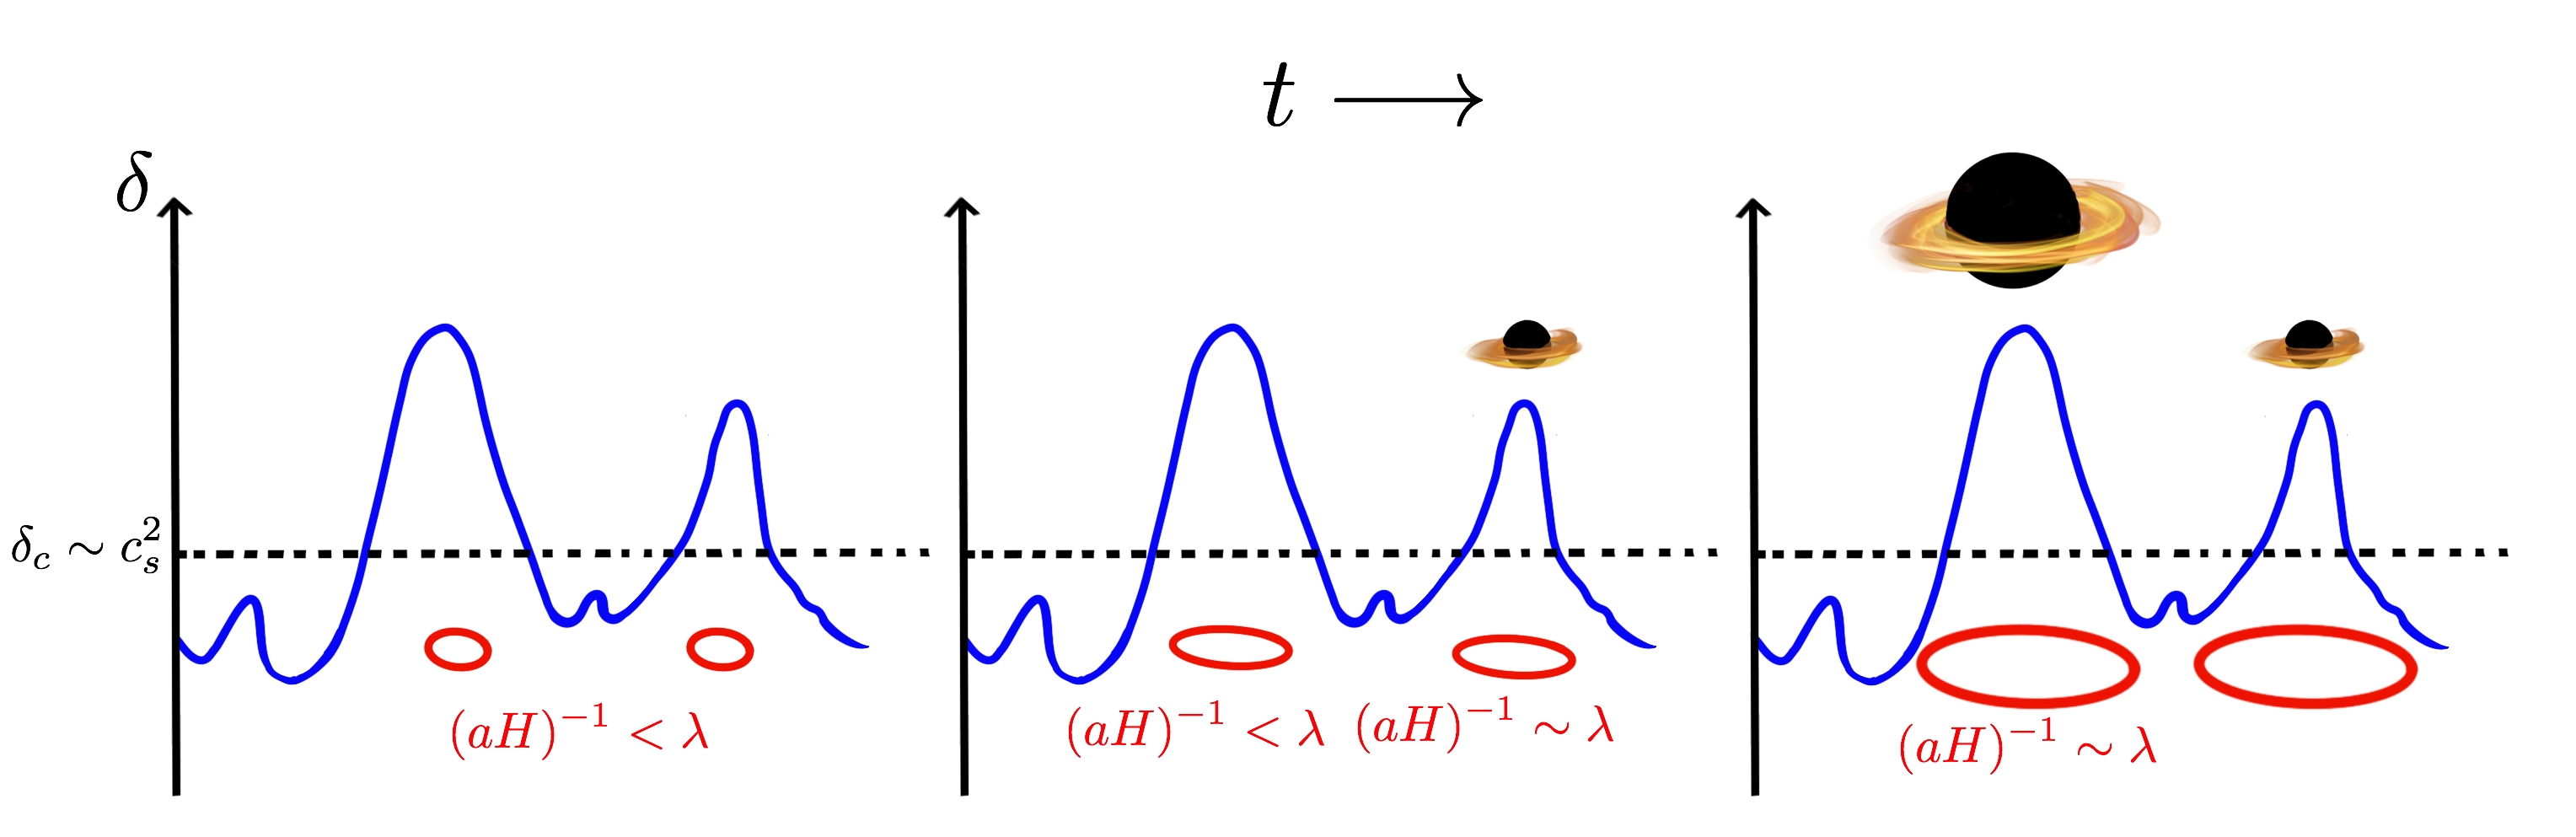
\includegraphics[scale=0.17]{Immagini/PBHformation.png}
			\caption{\small the later a perturbation crosses the horizon, the bigger the black hole. Figure from \cite{villanueva2021brief}.}
		\end{figure}
	\begin{itemize}
		\item Large inhomogeneities needed: \(\delta \ge \delta _c  \sim w = \frac{1}{3}\) \cite{osti_4109902}.
		\item {\small \(P(\delta)\) is gaussian} \(\implies\) \(\begin{cases}
		\beta(M) \sim \gamma \frac{\sigma(M)}{\delta_c}\exp\left(-\frac{\delta_c^2}{2\sigma(M)^2}\right) \ll 1\\
		\beta(M) \sim 10^{-8} \implies \Omega_{PBH}(t_0) \sim 1.
		\end{cases}
		\)
				%Deviations from the gaussian distribution are needed.
	\end{itemize}
	\end{frame}


\section{Constraints}



\begin{frame}
	\frametitle{Constraints on Evaporated PBHs}
	\begin{columns}
		\column{0.65\textwidth}
		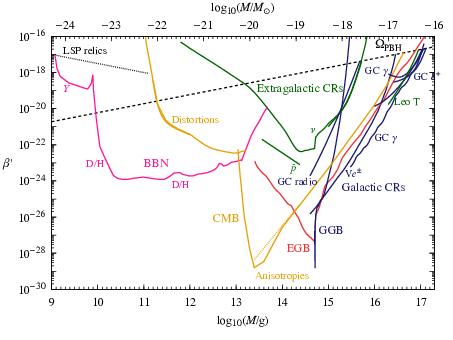
\includegraphics[scale=0.49]{Immagini/Evaporation.png}
		\begin{center}
			{\small\(\pumpkin\) A monochromatic mass function is assumed~\cite{Carr:2020gox}.}
		\end{center}
		
		\column{0.35\textwidth}
		\begin{itemize}
			\item \(\tau_{\text{Ev}} \propto M_{PBH}^3\).
			\item BBN: \(M\sim 10^{10}\si{\g}\) \(\implies \tau_{\text{Ev}} \sim \tau_{\text{BBN}}\)
				{\small change in the weak interaction freeze-out time and light elements abundances.}
			\item CMB: {\small spectrum distortion and small scales anisotropies damping.}
			\item EGB: {\small extragalactic \(\gamma\)-ray background.}
		\end{itemize}
	\end{columns}
	
\end{frame}

\begin{frame}
\frametitle{Constraints on non-evaporated PBHs}
\begin{columns}
	\column[t]{0.55\textwidth}
	%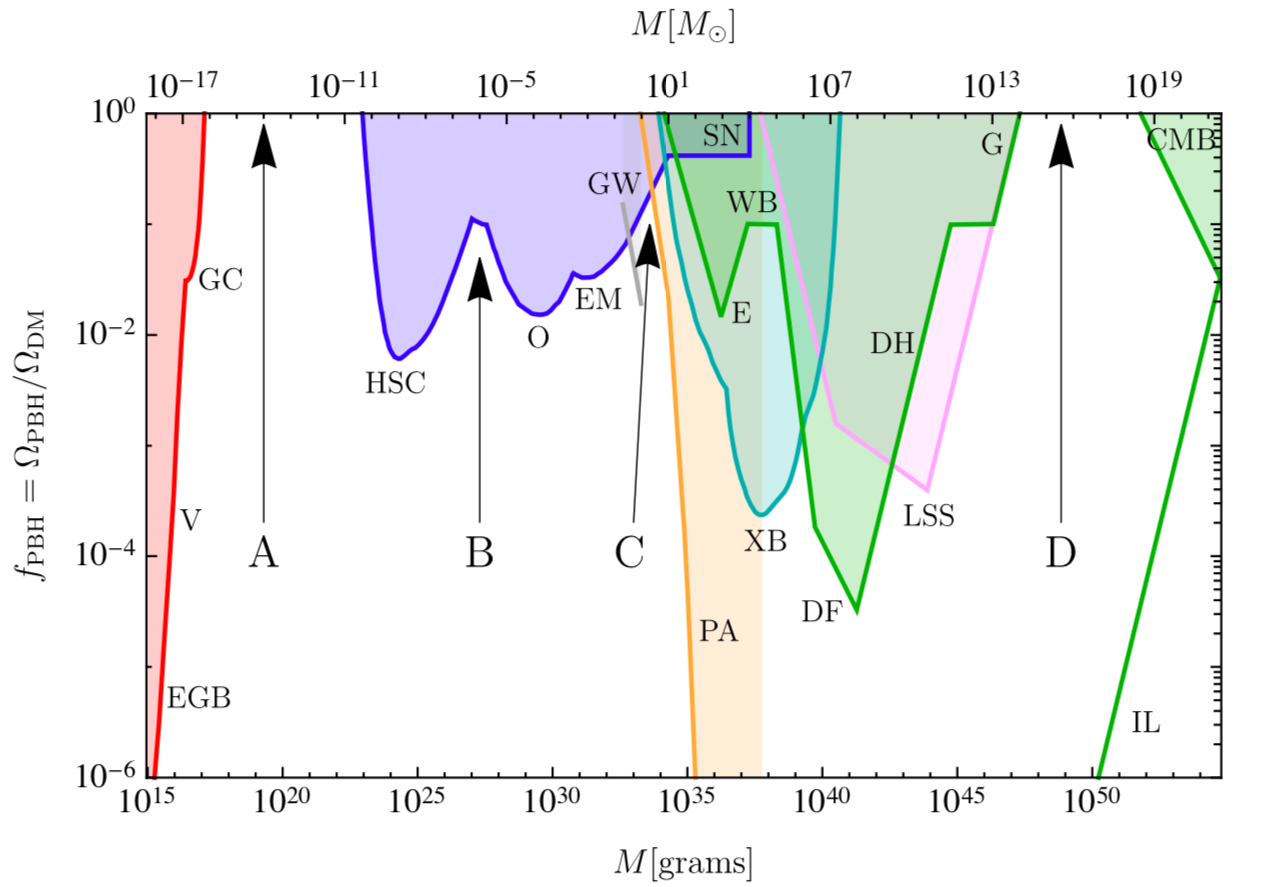
\includegraphics[scale=0.14]{Immagini/Constraints.png}
	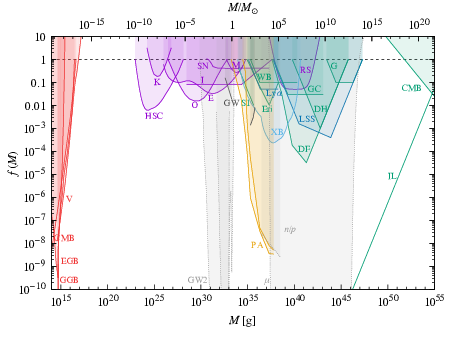
\includegraphics[scale=0.37]{Immagini/Updated_constr.png}
	\begin{itemize}
		\item<1-> \textbf{Evaporation:} \(M_{*} \sim 5 \times 10^{14}\si{\g}\).
		\item<2-> \textbf{Lensing:} searches for lensing events in galactic halos; \(95\%\) CL constraints.
	\end{itemize}
	\column{0.45\textwidth}
	\textbf{General assumptions~\cite{Carr:2020xqk}}
	\begin{itemize}
		\item PBH cluster in the same way as other forms of CDM.
		\item Monochromatic mass function: \(\Delta M \sim M\).
	\end{itemize}
	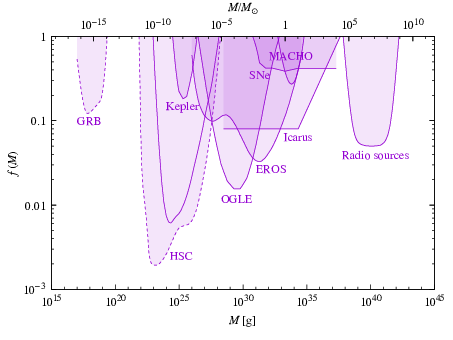
\includegraphics[scale=0.31]{Immagini/frac_lens.png}
\end{columns}
\end{frame}

\begin{frame}
	\begin{columns}
		\column{0.47\textwidth}
		\textbf{Dynamical constraints}:\cite{Carr:2020xqk}
		
		Objects are disrupted by nearby PBHs.
		\begin{itemize}
			\item Wide binaries;
			\item Galaxies halos;
			\item Dwarf galaxies.
		\end{itemize}
	Intergalactic PBHs induce a peculiar velocity:
	\[
	V_{pec}\sim \frac{GMt_0}{d^2}.
	\]
	
	\textbf{Accretion constraints:}\cite{Carr:2020xqk}
	PBHs accretion of background gas \(\leftrightarrow\) boost of matter temperature that reduces accretion and influences termal history.
	
	\column[t]{0.53\textwidth}
	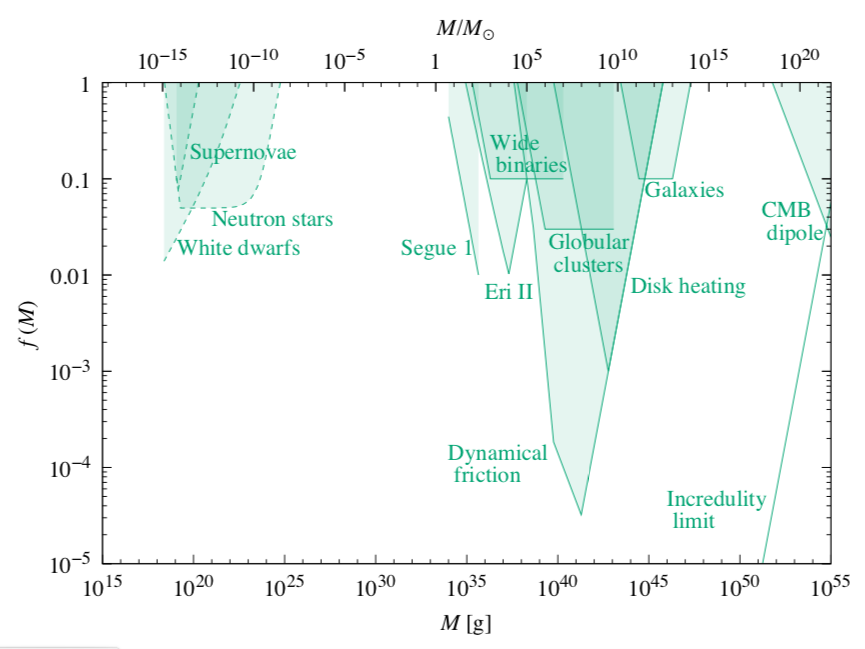
\includegraphics[scale=0.20]{Immagini/Dynamical.png}
	\vskip 7pt
	\textbf{\(\mu-\)distortion}
	
	Small scales density perturbations originates PBHs but are dissipated by Silk damping:
	
	\(\implies\) \(\mu-\)distortion in CMB spectrum: \(\delta(M) < \sqrt{\mu}\sim 10^{-2}\) for \(10^3 < \frac{M}{M_{\odot}} < 10^{12}\).
	\end{columns}
	
\end{frame}

\begin{frame}
	\frametitle{PBH binary formation \cite{Raidal:2017mfl}}
	\begin{columns}
		\column{0.75\textwidth}
		\textbf{Early formation}: at \(t\sim t_{eq}\). 
		\begin{itemize}
			\item negligible peculiar velocities;
			\item three-body approximation;
			\item \(\mathrightbat\) log-normal distribution: 
			\(\psi (m) = \frac{f_{PBH}}{\sqrt{2\pi}\sigma m}\exp\left(-\frac{\log^2(m/m_c)}{2\sigma^2}\right).\)
		\end{itemize}
	\textbf{Decoupling:} \(\frac{1}{2}(m_1 + m_2) > \frac{4\pi}{3}\rho_{bg}r^3 \implies a_{dc} \simeq a_{eq}\left(\frac{x}{\tilde{x}}\right)^3\).
	
	\centering	\(\Downarrow\)
	
{\small	\(dn_3(x,y) = \frac{1}{2}\left(\rho_{DM}\frac{\psi(m)}{m}dm_1\right)\left(e^{-N(y)} dN(x,m_2)dN(y,m_3) \right))\)

	\(dR_3(t) = \int_{0}^{\tilde{x}}dx\int_{x}^{\infty}dy \frac{\partial^2n_3}{\partial x\partial y}\delta(t - \tau(x,y,m_i))\).}
	
	\column{0.25\textwidth}
	\textbf{Late formation}: during non-linear phase of structure formation.
	\begin{itemize}
		\item Close encounters;
		\item Great loss of kinetic energy by friction or GWs.
	\end{itemize}
	\end{columns}
	
\end{frame}

\begin{frame}
	\frametitle{LIGO/Virgo observations}
	\textbf{Remark:} only a small fraction of PBH is in binaries.
	{\small\[
	R_3(t_0)\simeq 5.1\times 10^4
	 \delta_{dc}^{\frac{16}{37}}f_{PBH}^{\frac{53}{37}} \left(\frac{m_c}{30M_{\odot}}\right)^{-\frac{32}{37}}\si{\giga}pc^{-3}yr^{-1} \implies f_{PBH} \sim \mathcal{O}(10^{-2}).
	\]}
	\textbf{Stochastic GW background}:
	
	\[\Omega_{GW}(\nu) = \frac{\nu}{\rho_c}\int dzdR(z)\frac{1}{(1+z)H(z)} \frac{dE_{GW}(\nu_r)}{d\nu}\].
	
	\begin{columns}
		\column{0.34\textwidth}
		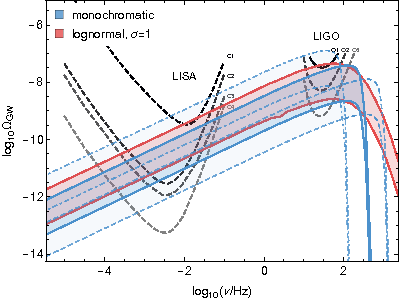
\includegraphics[scale=0.31]{Immagini/GWspectrum.png}
		\column{0.66\textwidth}
		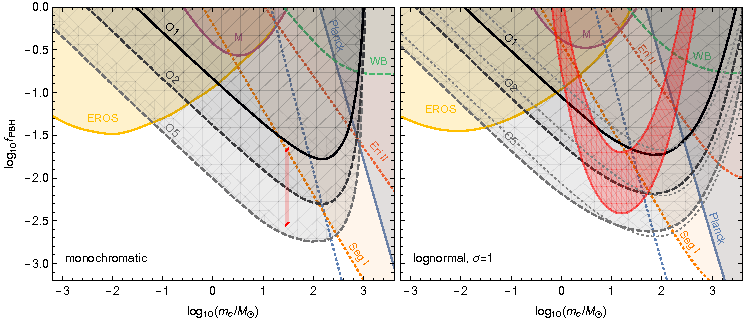
\includegraphics[scale=0.28]{Immagini/GWconstr.png}
	\end{columns}
\end{frame}

\begin{frame}
\frametitle{Mass windows \& comments}
	\begin{columns}
		
		\column{0.6\textwidth}
		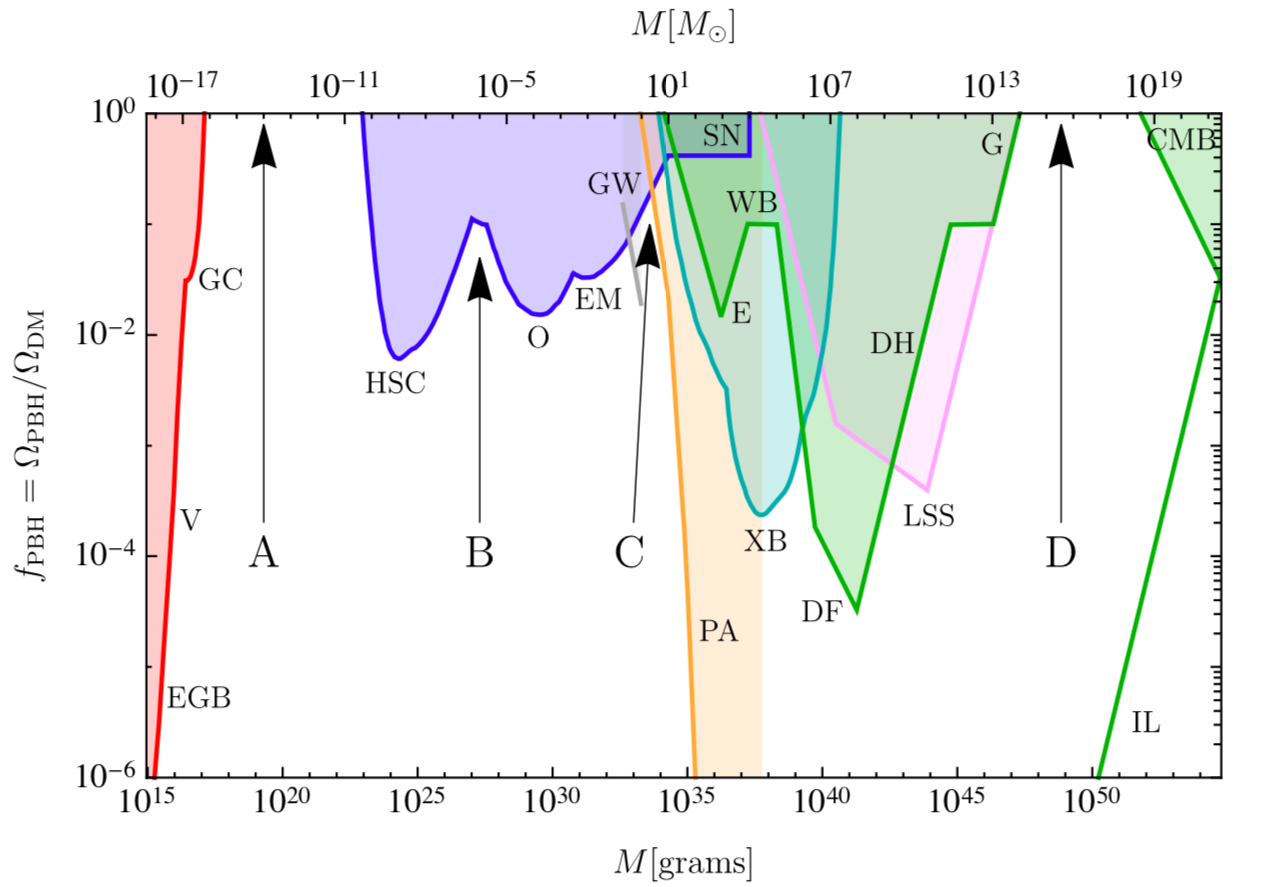
\includegraphics[scale=0.14]{Immagini/Constraints.png}
		\column{0.4\textwidth}
		\textbf{Window D}:
		\begin{itemize}
			\item {\small SLABs cannot be in galactic halos but could be \emph{intergalactic} DM.}
			\item {\small BH in GN have \(M\sim 10^{11}M_{\odot}\) but PBH are unlikely to be this large at formation.}
		\end{itemize}
		
	\end{columns}

{\small
\textbf{Extended mass function}

\begin{enumerate}
	\item<1-> \(\psi (M)\propto M\frac{dn}{dM}\) normalized with \(f_{PBH}\); \(\psi\) loc. specified by \(M_c\) and \(\sigma\).
	\item<2-> {\scriptsize \(A[\psi(M)] = A_0 + \int dM\psi(M)K_1(M) + \int dM_1dM_2\psi(M_1)\psi(M_2)K_2(M_1,M_2)+\ldots \)}
	\item<3-> \(A[\psi(M)]  \le A_{exp}\implies f_{PBH}(M_c) \le\frac{A_{exp} - A_0}{K_1(M_c)} := f_{max}(M_c)\).
	\item<4-> \(\int dM \frac{\psi(M)}{f_{max}(M)} \le 1\). Allowed mass range decreases with increasing \(\sigma\).
	
\end{enumerate}}
\end{frame}



\section{Claimed evidences}

\begin{frame}
	\frametitle{Lensing events}
	\begin{figure}
		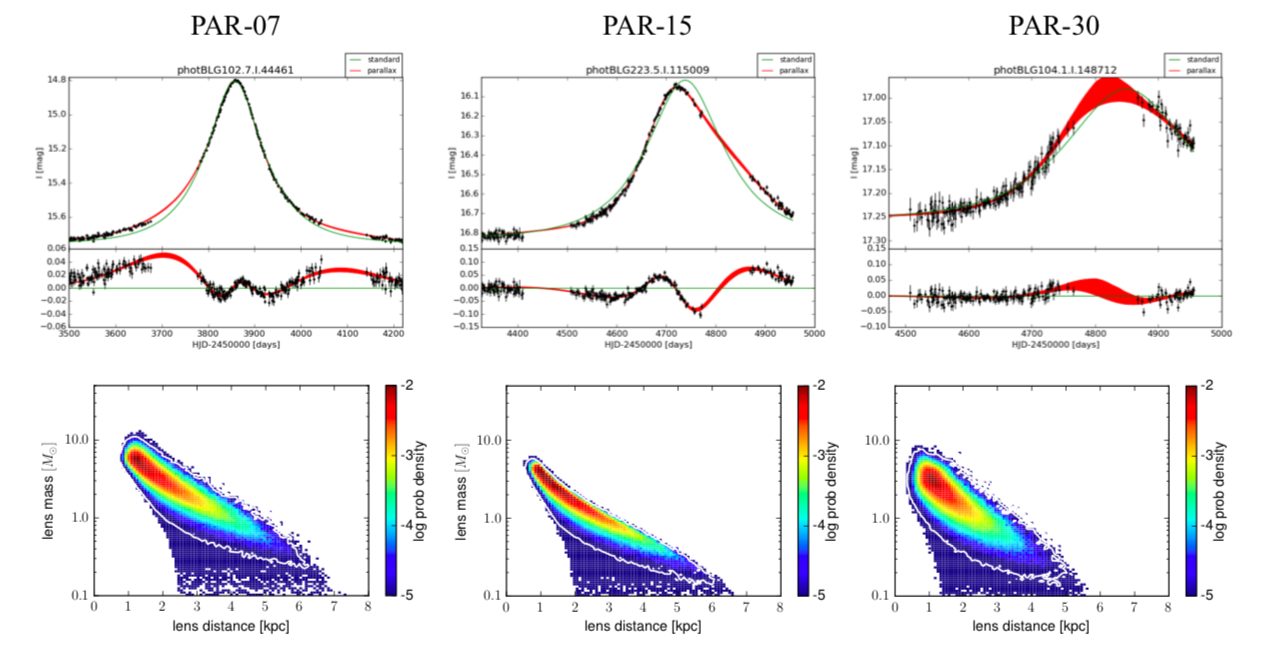
\includegraphics[scale=0.23]{Immagini/Lensing.png}
%		\caption{\tiny Microlensing events with mass estimates in the mass gap. Top panel: Light curves. Bottom panel: Mass-distance posterior probability densities along with the 95\% confidence level contour.}
	\end{figure}
	Among others OGLE\cite{Wyrzykowski_2020} has detected lensing events probably due to black holes, whose mass function peaks between \(0.8\) and \(5M_{\odot}\), overlapping with the mass gap of \(2-5M_{\odot}\) where black holes are not expected to form via gravitational collapse.
\end{frame}

\begin{frame}
	\frametitle{Ultra Faint Dwarf Galaxies \cite{Clesse:2017bsw}}
	\begin{figure}
		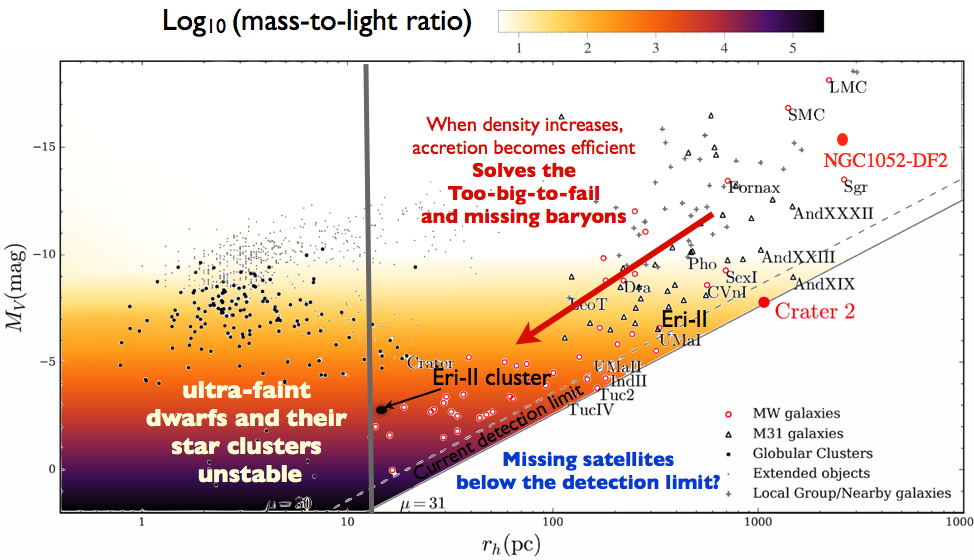
\includegraphics[scale=0.27]{Immagini/UFDG.png}
%		\caption{\tiny Absolute magnitude vs. the half-light ration of dwarf galaxies. Mass-to-light ratio based on toy model with uniform spherical halo with mass, radius and virial velocity relations calibrated on Eridanus II.}
	\end{figure}

	\begin{itemize}
		\item {\small Critical radius \(r_c \sim 10-20\) pc for dynamical heating of stars in \(1\si{\giga}\)yr coincides with minimal value observed.}
		%todo: capire che significa dynamical heated
		\item {\small Lack of luminous (especially large) dwarf galaxies: \emph{too-big-to-fail} problem. PBH accretion could prevent important star formation.}
	\end{itemize}
\end{frame}

\begin{frame}
	\frametitle{LIGO/Virgo observations}
	
	\begin{columns}
		\column{0.5\textwidth}
		\begin{figure}
			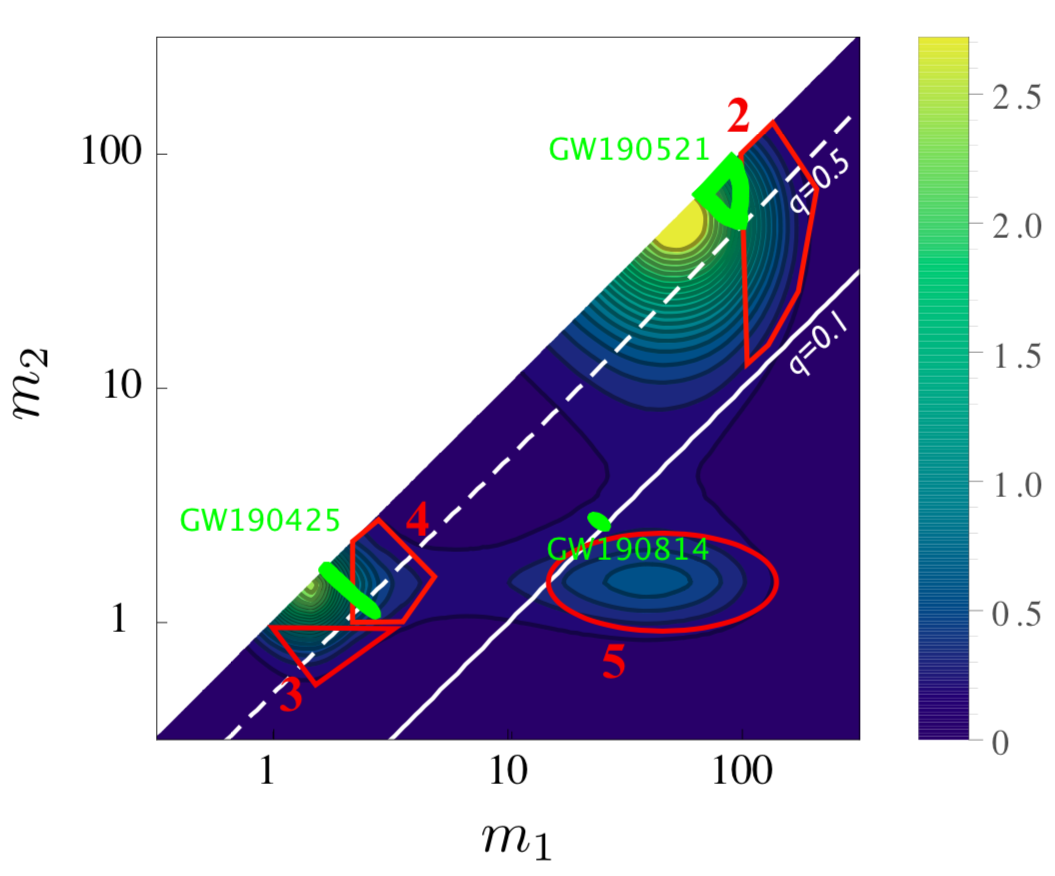
\includegraphics[scale=0.17]{Immagini/LIGO-Virgo.png}
			\caption{\scriptsize Merger of stellar black holes are not expected within the red bounded region. The colour bar indicates the probability of detection.}
		\end{figure}
		
		
		\column{0.5\textwidth}
		\begin{itemize}
			\item {\small Stellar Black Holes are expected to have non-negligible spin, while most of LIGO observations have effective spin compatible with 0.}
			\item {\small Raidal \textit{et al.} \cite{Raidal:2017mfl} show that PBHs can explain LIGO/Virgo observations without violating any current constraints, if they have a lognormal distribution function. They predict a gravitational wave background that can be observed by coming runs of LIGO.}
		\end{itemize}
	\end{columns}
\end{frame}
	


\begin{frame}
\centering

{\Huge \textcolor{blue}{Thank you for your attention!}}
\vskip 17pt
%\nocite{*}
\textbf{Bibliography}
\printbibliography
\end{frame}

\begin{frame}
\frametitle{Density Contrast threshold \cite{osti_4109902}}
Spherically symmetric perturbation:
\[
ds^2 = d\tau^2 - S^2\left[\frac{dr^2}{1-\kappa r^2} + r^2d\Omega^2\right]
\implies 
\begin{cases}
t_c \sim t_0\delta_0^{-\frac{3(1+f)}{2(1+3f)}}\\
S_c \sim R_0\delta_0^{-\frac{1}{(1+3f)}}
\end{cases}
\]
Condition for collapse:
\[
\sqrt{\frac{\pi w}{G\rho}} = \frac{2\pi}{k_J}< S_c < R_H \simeq \frac{1}{2H}
\]
\begin{block}{Collapse condition}
	\[1 > \delta_0 \left(\frac{R_0}{t_0}\right)^2 > w \sim \frac{1}{3}. \]
\end{block}
\centering
\(\mathrightghost\) Numerical simulations argue \(\delta_c \sim 0.45\) \(\mathleftghost\)
\end{frame}

\end{document}
